\section{Consuntivazione}

\subsection{Milestones:}
\begin{itemize}
    \item Release versione 0.0.4 dell'analisi dei requisiti(Completa al: 100\%)
    \item Release versione 0.0.5 dell'analisi dei requisiti(Completa al: 60\%)
\end{itemize}

\subsection{Attività svolte}

\begin{table}[H]
    \begin{xltabular}{\textwidth}{X l l}
        
        \rowcolor{gray!30} \textbf{Attività} & \textbf{Stato} & \textbf{Ruolo}\\
        \endhead
        \hline
        riviste e riorganizzate tutte le uc & completato & Analista \\
        rilasciata versione 0.0.4 dell'analisi dei requisiti & completato & Responsabile \\
    \end{xltabular}
    \caption{Lista delle attività svolte durante lo sprint}
\end{table}


\begin{table}[ht]
    \begin{tabularx}{\linewidth}{X|rrrrrrr}
    \rowcolor{gray!30}& Re & Amm & An & Pro & Prog & Ver & tot \\
    \hline
    Bonavigo Michele                        & 1,5 & 0 & 3,15 & 0 & 0 & 1,75  & 6,4 \\
    \rowcolor{gray!10}Casarotto Mattia      & 0 & 0 & 1,65 & 0 & 0 & 0 & 1,65 \\
    Massarenti Alessandro                   & 3,3 & 0 & 0,9 & 0 & 0 & 0,6  & 4,8 \\
    \rowcolor{gray!10}Peron Samuel          & 0 & 0 & 0 & 0 & 0 & 0 & 0 \\
    Pierobon Luca                           & 0 & 0 & 0 & 0 & 0 & 3,3 & 3,3 \\
    \rowcolor{gray!10}Romano Davide         & 0 & 0 & 0 & 0 & 0 & 0 & 0 \\
    Zarantonello Giorgio                    & 0 & 0 & 1,75 & 0 & 0 & 0 & 1,75 \\
    \hline                                  & 4,8 & 0 & 7,45 & 0 & 0 & 5,65 & \\
    \end{tabularx}
    \caption{\label{ruoli-persone}Spartizione dei ruoli e ore svolte durante lo sprint}
\end{table}

\begin{center}
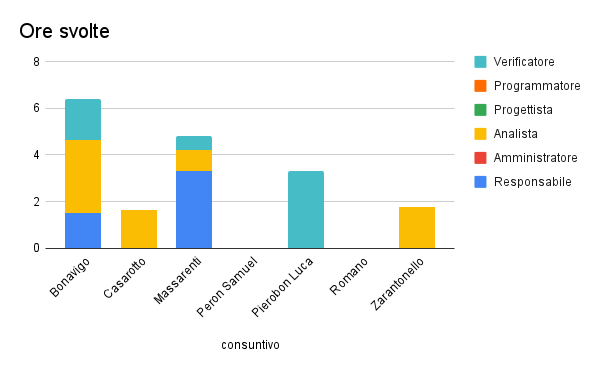
\includegraphics[width=12cm]{img/ore-svolte.png}
\end{center}

\begin{table}[ht]
    \begin{tabularx}{\linewidth}{X|l|l}
    \rowcolor{gray!30}& Ore & Costo \\
    \hline
    
    Responsabile & 4,8 & € 144,00 \\
    \rowcolor{gray!10}Amministratore & 0 & € 0,00 \\
    Analista & 7,45 & € 186,25 \\
    \rowcolor{gray!10}Progettista & 0 & € 0,00 \\
    Programmatore & 0 & € 0,00 \\
    \rowcolor{gray!10}Verificatore & 5,65 &€ 84,75 \\
    totale & 17,9 & € 415,00 \\
    \end{tabularx}
    \caption{\label{costi-ruolo}Spartizione dei ruoli e ore svolte durante lo sprint}
\end{table}

Avendo quindi consumato €415,00\footnote{Si veda tabella \ref{costi-ruolo}} del budget durante questo sprint, rimangono ancora a disposizione € 11372,50 per gli sprint seguenti.

\subsection{Trend e riflessioni}

\begin{figure}[H]
    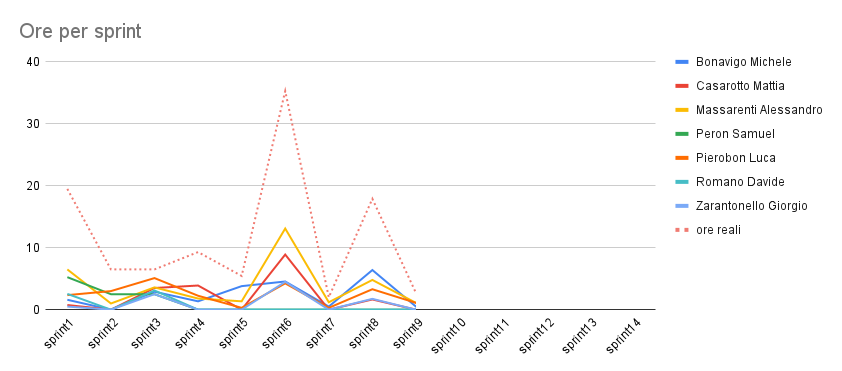
\includegraphics[width=\linewidth]{img/andamento.png}
    \caption{Andamento ore utilizzate nei vari sprint}\label{img:andamento}
\end{figure}

Dopo aver notato nello sprint precedente come il mettere in coda le attività di progetto non sia costruttivo, il gruppo ha lavorato per aumentare il ritmo.

È desiderio del gruppo continuare a lavorare su questo aspetto.

\subsection{Difficoltà e problemi di sprint}

Non ci sono state grandi difficoltà esterne durante questo sprint. Purtroppo però, come negli sprint appena precedenti, non siamo ancora riusciti a definire con il proponente il supporto hardware per i lampioni a cui dovremo fare fede.

Nonostante il gruppo abbia lavorato per aumentare il ritmo, questa tendenza non è stata seguita da tutti i membri. Si può notare in figura \ref{img:andamento} come alcuni membri non abbiano migliorato il loro trend non partecipativo iniziato nello sprint 4.

Queste verranno discusse in sede di preparazione del prossimo sprint.
